\section{Neural Geometry Fields (NGFs)}\label{Sec:MainPart}

Sivaram and colleagues divide the Neural Geometry Fields pipeline into three distinct stages.

First, they input a base mesh \( \Sigma \) and partition it into quadrangular patches.
From this, they construct a trainable feature field \( \Psi : \Sigma \to \mathbb{R}^F \), associating each patch with a set of features that describe its surface properties, where each feature consists of \( F \) real components.
In the second stage, they feed these features, along with the 3D positions of the mesh, into a neural network that computes the displacement for each point on the mesh.
They then apply the displacements to the base mesh, producing a transformed conventional triangle mesh.
Finally, they optimize the feature field and patches using an inverse rendering algorithm.

In the following sections, we explore each stage in greater detail and provide an example to clarify the process further.






\subsection{Surface Partitioning into Patches}

Sivaram and colleagues introduce a method for surface representation by partitioning a base mesh, denoted as $\Sigma$, into quadrilateral patches $\sigma$ (see Figure~2).  
The process begins by simplifying the input mesh using QSlim, a robust and scalable algorithm that preserves important topological features such as holes and intersections.  
Following simplification, adjacent triangles are greedily merged into near-rectangular quadrilaterals, removing non-manifold triangles in the process.  
This allows the method to handle non-manifold input surfaces and still produce a consistent quadrilateral patch structure.  
This produces a compact and regular representation of the surface geometry, with fewer patches and improved structure.  
\usetikzlibrary{calc, shapes.geometric, arrows.meta, decorations.pathreplacing, positioning, shapes}
\begin{figure}[ht]
  \centering
  \begin{adjustbox}{center}
  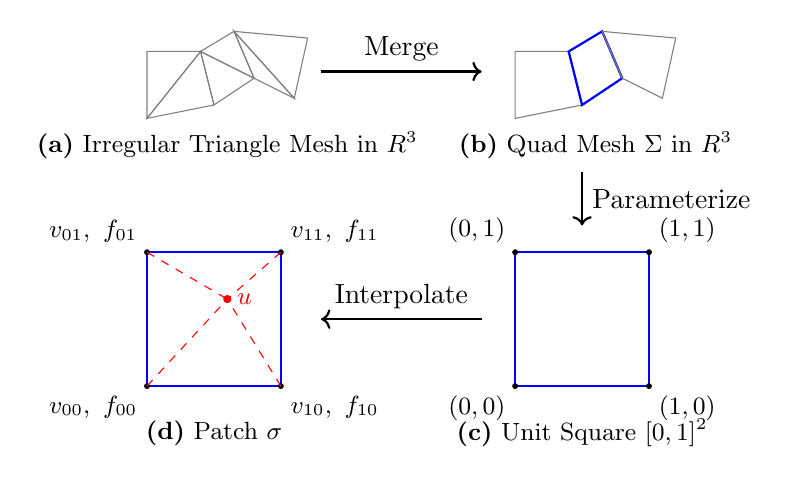
\begin{tikzpicture}[scale=0.85]

    % === Triangle Mesh (Left) ===
    \begin{scope}
      \coordinate (A) at (0,0);
      \coordinate (B) at (1,0.2);
      \coordinate (C) at (0.8,1);
      \coordinate (D) at (0,1);
      \coordinate (E) at (1.6,0.6);
      \coordinate (F) at (1.3,1.3);
      \coordinate (G) at (2.2,0.3);
      \coordinate (H) at (2.4,1.2);

      \draw[gray] (A) -- (B) -- (C) -- cycle;
      \draw[gray] (A) -- (C) -- (D) -- cycle;
      \draw[gray] (B) -- (E) -- (C) -- cycle;
      \draw[gray] (C) -- (E) -- (F) -- cycle;
      \draw[gray] (E) -- (G) -- (F) -- cycle;
      \draw[gray] (F) -- (G) -- (H) -- cycle;
      \node at (1.2, -0.4) {\small \textbf{(a)} Irregular Triangle Mesh in $\mathbb{R}^3$};
    \end{scope}

    % === Merge Arrow ===
    \draw[->, thick] (2.6,0.7) -- (5.0,0.7) node[midway, above] {Merge};

    % === Quadrilateral Mesh (Middle) ===
    \begin{scope}[xshift=5.5cm]
      \coordinate (A) at (0,0);
      \coordinate (B) at (1,0.2);
      \coordinate (C) at (0.8,1);
      \coordinate (D) at (0,1);
      \coordinate (E) at (1.6,0.6);
      \coordinate (F) at (1.3,1.3);
      \coordinate (G) at (2.2,0.3);
      \coordinate (H) at (2.4,1.2);

      \draw[gray] (A) -- (B) -- (C) -- (D) -- cycle;
      \draw[blue, thick] (B) -- (E) -- (F) -- (C) -- cycle; % highlighted patch
      \draw[gray] (E) -- (G) -- (H) -- (F) -- cycle;

      \node at (1.2, -0.4) {\small \textbf{(b)} Quad Mesh $\Sigma$ in $\mathbb{R}^3$};
    \end{scope}

    % === Down Arrow to Unit Square ===
    \draw[->, thick] (6.5,-0.8) -- (6.5,-1.6) node[midway, right] {Parameterize};

    % === Unit Square (Right) ===
    \begin{scope}[xshift=5.5cm, yshift=-4.0cm]
      \draw[blue, thick] (0,0) rectangle (2,2);
      \filldraw[black] (0,0) circle (1pt) node[anchor=north east] {\small $(0,0)$};
      \filldraw[black] (2,0) circle (1pt) node[anchor=north west] {\small $(1,0)$};
      \filldraw[black] (0,2) circle (1pt) node[anchor=south east] {\small $(0,1)$};
      \filldraw[black] (2,2) circle (1pt) node[anchor=south west] {\small $(1,1)$};
      \node at (1,-0.7) {\small \textbf{(c)} Unit Square $[0,1]^2$};
    \end{scope}

    % === Left Arrow to Feature Field ===
    \draw[->, thick] (5.0,-3) -- (2.6,-3) node[midway, above] {Interpolate};

    % === Feature Field (Left) ===
    \begin{scope}[yshift=-4.0cm]
      \draw[blue, thick] (0,0) rectangle (2,2);

      % Corner features (bold vectors), with f00 label moved outward
      \filldraw[black] (0,0) circle (1pt) node[anchor=north east] {\small $\bm{v_{00}},\ \bm{f_{00}}$};
      \filldraw[black] (2,0) circle (1pt) node[anchor=north west] {\small $\bm{v_{10}},\ \bm{f_{10}}$};
      \filldraw[black] (0,2) circle (1pt) node[anchor=south east] {\small $\bm{v_{01}},\ \bm{f_{01}}$};
      \filldraw[black] (2,2) circle (1pt) node[anchor=south west] {\small $\bm{v_{11}},\ \bm{f_{11}}$};

      % Interpolation point (u)
      \filldraw[red] (1.2,1.3) circle (1.5pt) node[right] {\small $\bm{u}$};

      % Lines from corners to interpolation point
      \foreach \x/\y in {0/0, 2/0, 0/2, 2/2} {
        \draw[dashed, red] (\x,\y) -- (1.2,1.3);
      }

      % Patch label
      \node at (1,-0.7) {\small \textbf{(d)} Patch $\sigma$};
    \end{scope}
    
  \end{tikzpicture}
  \end{adjustbox}
  \caption{Surface processing pipeline: The irregular triangle mesh is simplified and merged into a quadrilateral mesh $\Sigma$. A quadrilateral patch is extracted, which is then parameterized over the unit square $[0,1]^2$. This parameterization facilitates both geometric and feature field interpolation, with feature values interpolated at the patch's corners and at an arbitrary point $\bm{u}$. Inspired by~\cite{sivaram2024}.}
  \label{fig:surface_processing_pipeline}
\end{figure}
By relying on quadrilateral patches instead of a fully triangulated mesh, the method reduces the overall patch count $|Q|$ and simplifies the interpolation domain for later processing.  
This compression not only reduces storage requirements but also provides the foundation for an efficient and structured interpolation framework.  

To ensure smooth and consistent interpolation, each patch $\sigma$ must be diffeomorphic to the unit square $[0,1]^2$, meaning there exists a smooth, bijective mapping with a smooth inverse between the patch and the unit square.  
The four corner vertices of a patch are mapped as:
\[(0,0)\rightarrow v_{00}, \quad (1,0)\rightarrow v_{10}, \quad (0,1)\rightarrow v_{01}, \quad (1,1)\rightarrow v_{11}\]

To map an arbitrary point $u = (u_x, u_y)$ within the unit square to its corresponding location on the surface patch $\sigma$, bilinear interpolation is applied:  
\[\sigma(u) = (1 - u_y)((1 - u_x)v_{00} + u_x v_{10}) + u_y((1 - u_x)v_{01} + u_x v_{11}) \tag{1}\]  
This yields a continuous and smooth surface.  
Conceptually, this bilinear interpolation can be thought of as first interpolating along one axis (e.g., horizontal), then the other.  
The same interpolation strategy is used to propagate feature vectors defined at each patch corner.  

Each patch corner is associated with a high-dimensional learnable feature vector.  
In the configuration used by Sivaram et al., each vector has 20 dimensions, acting as a localized descriptor of geometric or semantic properties.  
The interpolated feature value $\Psi(u)$ for a point $u$ inside a patch is computed using bilinear blending:  
\[\Psi(u) = (1 - u_y)((1 - u_x)f_{00} + u_x f_{10}) + u_y((1 - u_x)f_{01} + u_x f_{11}) \tag{2}\]

The feature field $\Psi: \Sigma \rightarrow \mathbb{R}^F$ (with $F = 20$ in the authors' setup) allows the model to smoothly interpolate semantic information across the surface.  
These features, interpolated at arbitrary points on the patch, can be sampled across the surface for later neural processing stages.  

The complete set of mesh vertices and their associated features is defined as:  
\[V = \bigcup_\sigma \{v_{00}, v_{10}, v_{01}, v_{11}\}, \quad F = \bigcup_\sigma \{f_{00}, f_{10}, f_{01}, f_{11}\}\]  

These values are bilinearly interpolated across each patch and serve as input for the subsequent neural deformation stage.  
The surface layout defined in this step provides a structured yet flexible representation that supports efficient learning and reconstruction.  

The following section describes how this patch-based representation is used to generate detailed geometry through a neural deformation model, including the role of tessellation, feature encoding and the architecture of the MLP.  





\subsection{Patch-Based Sampling and Feature Encoding}

Building on the quadrilateral patch structure introduced before, Sivaram et al.\ develop a neural representation that enables fine-grained geometry reconstruction over this base mesh.
Each patch, defined as a bilinear map from the unit square $[0,1]^2$ to a region on the simplified surface, provides a consistent local domain for both geometric interpolation and neural processing.

To capture detailed shape variations across the surface, the method samples a dense grid of points within each patch.
A regular $k \times k$ grid is overlaid on the unit square domain, producing a set of parametric coordinates $u_{ij} \in [0,1]^2$ for $i,j \in \{0,\ldots,k-1\}$.
These samples form the foundation for evaluating both geometry and features across the patch.

At each sample location $u_{ij}$, two quantities are computed: 

\quad $\bullet$ The 3D position $\sigma(u_{ij})$,

\quad $\bullet$ The interpolated feature vector $\Psi(u_{ij})$.

To enable the network to learn surface deformations, the sampled geometry and feature values are transformed through a high-frequency positional encoding~\cite{mildenhall2020}.
Specifically, each input point is encoded as: 
\[\text{enc}(v,f) = (\sin(2^0 v), \cos(2^0 v), \ldots, \sin(2^L v), \cos(2^L v), f)\]
where $v = \sigma(u)$, $f = \Psi(u)$ and $L = 8$ defines the number of frequency bands.
This encoding combines geometric location with semantic features in a form suitable for learning complex local surface variations.

The result is a structured and differentiable input representation that supports the subsequent neural deformation process.
\begin{figure}[ht]
  \centering
  \begin{adjustbox}{center}
  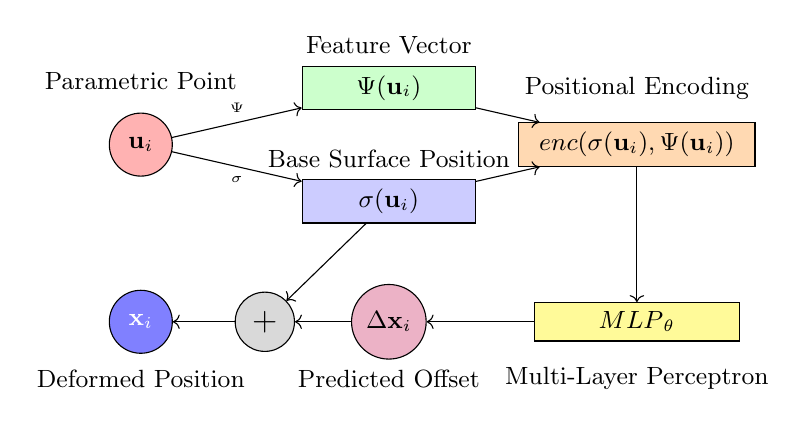
\begin{tikzpicture}[scale=0.9]

    % Sample point u_i
    \node[draw, circle, fill=red!30, minimum size=0.8cm] (u) at (0,0) {\small $\mathbf{u}_i$};
    \node at (0,0.9) {\small Parametric Point};

    % Psi(u)
    \node[draw, rectangle, fill=green!20, minimum width=2.2cm] (psi) at (3.5,0.8) {\small $\Psi(\mathbf{u}_i)$};
    \node at (3.5,1.4) {\small Feature Vector};

    % Sigma(u)
    \node[draw, rectangle, fill=blue!20, minimum width=2.2cm] (sigma) at (3.5,-0.8) {\small $\sigma(\mathbf{u}_i)$};
    \node at (3.5,-0.2) {\small Base Surface Position};

    % Encoding node
    \node[draw, rectangle, fill=orange!30, minimum width=3cm] (enc) at (7,0) {\small $\text{enc}(\sigma(\mathbf{u}_i), \Psi(\mathbf{u}_i))$};
    \node at (7,0.8) {\small Positional Encoding};

    % MLP node
    \node[draw, rectangle, fill=yellow!40, minimum width=2.6cm] (mlp) at (7,-2.5) {\small $\text{MLP}_\theta$};
    \node at (7,-3.3) {\small Multi-Layer Perceptron};

    % Displacement vector
    \node[draw, circle, fill=purple!30, minimum size=0.8cm] (dx) at (3.5,-2.5) {\small $\Delta \mathbf{x}_i$};
    \node at (3.5,-3.3) {\small Predicted Offset};

    % Plus node for summing sigma(ui) and delta_x (smaller + symbol)
    \node[draw, circle, fill=gray!30, minimum size=0.6cm] (plus) at (1.75,-2.5) {\large $+$};

    % Final position
    \node[draw, circle, fill=blue!50, text=white, minimum size=0.8cm] (x) at (0,-2.5) {\small $\mathbf{x}_i$};
    \node at (0,-3.3) {\small Deformed Position};

    % Arrows
    \draw[->] (u) -- (psi) node[midway, above] {\tiny $\Psi$};
    \draw[->] (u) -- (sigma) node[midway, below] {\tiny $\sigma$};
    \draw[->] (sigma) -- (enc);
    \draw[->] (psi) -- (enc);
    \draw[->] (enc) -- (mlp);
    \draw[->] (mlp) -- (dx);
    \draw[->] (sigma) -- (plus);
    \draw[->] (dx) -- (plus);
    \draw[->] (plus) -- (x);

  \end{tikzpicture}
  \end{adjustbox}
  \caption{Neural displacement pipeline for a sampled point $\mathbf{u}_i$. The point is mapped to a corresponding feature vector $\Psi(\mathbf{u}_i)$ and a base surface position $\sigma(\mathbf{u}_i)$. These inputs are passed through a positional encoding and a learned MLP to produce a displacement vector $\Delta \mathbf{x}_i$. The final deformed position $\mathbf{x}_i$ is obtained by adding the base position and the predicted offset, shown by the plus symbol.}
  \label{fig:neural_displacement}
\end{figure}





\subsubsection{Neural Surface Deformation with MLP}

Surface reconstruction is achieved by predicting local displacements using an MLP, which is conditioned on encoded geometric and feature information.
The deformed 3D point $\Lambda(u)$ is computed as:
\[\Lambda(u) = \sigma(u) + \text{MLP}_{\theta}(\text{enc}(\sigma(u), \Psi(u)))\]
This enables each point on the base mesh to undergo a locally adaptive deformation, refining the coarse patch approximation to recover high-fidelity geometry.





\subsubsection{Objective Function}

Unlike traditional pipelines that rely solely on image supervision, this method also utilizes ground truth geometric information — specifically, surface normal as a guiding signal.
Vertex normals are computed on the predicted mesh using cross products of adjacent triangle edges.
During differentiable rasterization, these per-vertex normals are interpolated across pixels to produce normal buffers for both the predicted surface $\Sigma$ and the reference surface $\Gamma$.
The image-space normal consistency loss is then defined as:
\[\mathcal{L}_{\text{normal}} = \frac{1}{|\mathcal{N}(\cdot)|} \left\| \mathcal{N}(\Gamma) - \mathcal{N}(\Sigma) \right\|_1\]

To promote smooth, uniform geometry and prevent artifacts like vertex clustering, a Laplacian regularization term is added:
\[\mathcal{L}_{\text{laplacian}} = \frac{1}{|V|} \left\| \mathcal{L}_V \right\|_1\]
where $\mathcal{L}$ is the uniform mesh Laplacian operator applied to the set of sampled vertices $V$.

The total loss function is:
\[\mathcal{L}_{\text{total}} = \mathcal{L}_{\text{normal}} + \mathcal{L}_{\text{laplacian}}\]

This formulation encourages the reconstructed mesh to be both visually accurate and structurally regular.





\subsubsection{Jittered Sampling for Detail and Regularization}

To enhance surface detail and training stability, Sivaram et al.\ employ jittered sampling, perturbing grid points within each patch.
While regular sampling places samples at evenly spaced positions $\hat{u} = \langle i,j \rangle / (k - 1)$, this uniformity can cause aliasing and oversmoothing, especially on high-frequency geometry.

To address this, interior sample points are offset by small, random perturbations from a disk-shaped distribution:
\[u \sim \hat{u} + D(\omega)\]
where $D(\omega)$ samples uniformly from a disk of radius $\omega$, introducing local variation while preserving patch structure.

To ensure mesh consistency: 

\quad $\bullet$ Boundary points are not jittered ($\omega = 0$) to preserve alignment between adjacent patches.

\quad $\bullet$ The jitter radius $\omega$ is constrained: $\omega < \frac{0.5}{k - 1}$, preventing triangle fold-overs or inversions.

\begin{figure}[ht]
  \centering
  \begin{adjustbox}{center}
  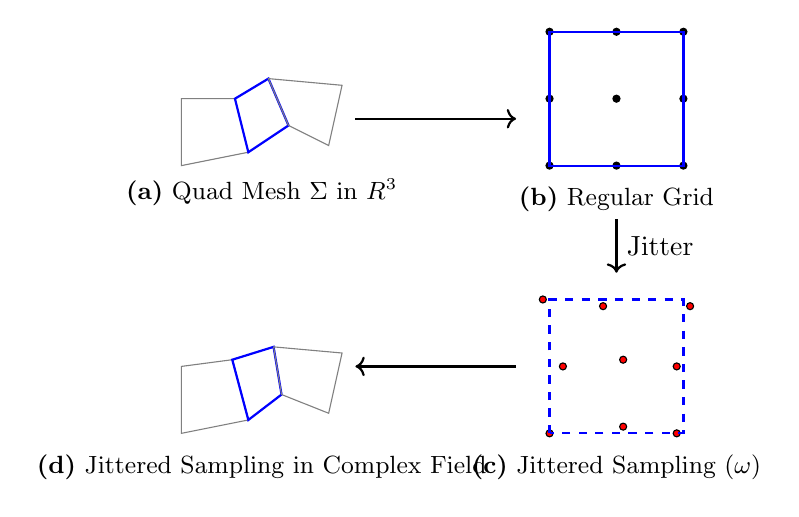
\begin{tikzpicture}[scale=0.85]

    % === (a) Irregular Triangle Mesh ===
    \begin{scope}
      \coordinate (A) at (0,0);
      \coordinate (B) at (1,0.2);
      \coordinate (C) at (0.8,1);
      \coordinate (D) at (0,1);
      \coordinate (E) at (1.6,0.6);
      \coordinate (F) at (1.3,1.3);
      \coordinate (G) at (2.2,0.3);
      \coordinate (H) at (2.4,1.2);

      \draw[gray] (A) -- (B) -- (C) -- (D) -- cycle;
      \draw[blue, thick] (B) -- (E) -- (F) -- (C) -- cycle; % highlighted patch
      \draw[gray] (E) -- (G) -- (H) -- (F) -- cycle;

      \node at (1.2, -0.4) {\small \textbf{(a)} Quad Mesh $\Sigma$ in $\mathbb{R}^3$};
    \end{scope}

    % Arrow
    \draw[->, thick] (2.6,0.7) -- (5.0,0.7) node[midway, above] {};

    % === (b) Regular Grid ===
    \begin{scope}[xshift=5.5cm]
      \foreach \x in {0,1,2} {
        \foreach \y in {0,1,2} {
          \filldraw[black] (\x, \y) circle (1.5pt);
        }
      }

      \draw[blue, thick] (0,0) rectangle (2,2);
      \node at (1,-0.5) {\small \textbf{(b)} Regular Grid};
    \end{scope}

    % Arrow
    \draw[->, thick] (6.5,-0.8) -- (6.5,-1.6) node[midway, right] {Jitter};

    % === (c) Jittered Grid ===
    \begin{scope}[xshift=5.5cm, yshift=-4.0cm]
      \foreach \x/\y in {
        0.0/0.0, 1.1/0.1, 1.9/0.0, 0.2/1.0,
        2.1/1.9, 1.1/1.1, 1.9/1.0, -0.1/2.0,
        0.8/1.9
      } {
        \filldraw[red, draw=black] (\x, \y) circle (1.5pt);
      }

      \draw[blue, thick, dashed] (0,0) rectangle (2,2);
      \node at (1,-0.5) {\small \textbf{(c)} Jittered Sampling ($\omega$)};
    \end{scope}

    % Arrow
    \draw[->, thick] (5.0,-3) -- (2.6,-3) node[midway, above] {};

    % === (d) Irregular Field + Jittered Points ===
    \begin{scope}[yshift=-4.0cm]
      
  \coordinate (A) at (0,0);
  \coordinate (B) at (1.000,0.200); %(1,0.2.0)
  \coordinate (C) at (0.760,1.100); %(0.8,1.0)
  \coordinate (D) at (0,1);
  \coordinate (E) at (1.496,0.580); %(1.6,0.6)
  \coordinate (F) at (1.377,1.292); %(1.3,1.3)
  \coordinate (G) at (2.2,0.3);
  \coordinate (H) at (2.4,1.2);

  \draw[gray] (A) -- (B) -- (C) -- (D) -- cycle;
  \draw[blue, thick] (B) -- (E) -- (F) -- (C) -- cycle; % highlighted patch
  \draw[gray] (E) -- (G) -- (H) -- (F) -- cycle;


  % === Jittered Points Mapped from (c) ===
  %\filldraw[red, draw=black] (1.000,0.200) circle (1.5pt); % (0.0, 0.0)
  %\filldraw[red, draw=black] (1.307,0.385) circle (1.5pt); % (1.1, 0.1)
  %\filldraw[red, draw=black] (1.496,0.580) circle (1.5pt); % (1.9, 0.0)
  %\filldraw[red, draw=black] (0.905,0.700) circle (1.5pt); % (0.2, 1.0)
  %\filldraw[red, draw=black] (1.377,1.292) circle (1.5pt); % (2.1, 1.9)
  %\filldraw[red, draw=black] (1.222,0.885) circle (1.5pt); % (1.1, 1.1)
  %\filldraw[red, draw=black] (1.450,0.880) circle (1.5pt); % (1.9, 1.0)
  %\filldraw[red, draw=black] (0.760,1.100) circle (1.5pt); % (-0.1, 2.0)
  %\filldraw[red, draw=black] (1.091,1.080) circle (1.5pt); % (0.8, 1.9)

  \node at (1.2, -0.5) {\small \textbf{(d)} Jittered Sampling in Complex Field};
\end{scope}


  \end{tikzpicture}
  \end{adjustbox}
  \caption{Progression from an irregular triangle mesh (a) to a regular sampling grid (b), jittered sampling within grid cells (c) and finally applying jittered sampling within a more complex field (d).}
  \label{fig:progression_sampling}
\end{figure}

This stochastic sampling improves generalization by preventing overfitting to a fixed grid layout.
It encourages smoother deformations and higher robustness, particularly in low-resolution regimes where fewer samples may otherwise miss fine geometric details.
As shown in Figure 4, jittered sampling yields cleaner, more accurate reconstructions compared to regular sampling.





\subsubsection{Mesh Construction and Differentiable Training}

Once deformed 3D positions are computed via the MLP, the mesh is formed by triangulating the $k \times k$ sampling grid within each patch.
Each square cell is split into two triangles in a consistent pattern, producing a semi-regular, watertight surface due to shared boundary vertices and uniform sampling logic.

The neural deformation network consists of an MLP with two hidden layers of 64 units each.
While the activation functions are not specified, they introduce the non-linearity required for complex deformations.
Both the MLP weights $\theta$ and the per-vertex feature vectors are optimized jointly.

Training leverages differentiable rendering via NVDIFFRAST~\cite{niemeyer2020}, enabling image-space gradients to flow back to both geometry and features.
This gradient-based feedback from multi-view supervision allows the model to iteratively refine the reconstructed surface.

To provide dense supervision, the model is rendered from 200 virtual viewpoints distributed uniformly around the object.
Each view is rendered with three depth layers per pixel to handle occlusions and transparency effects.
Views are processed in batches of 10 to balance memory and performance.

Optimization uses the Adam optimizer~\cite{kingma2017} with a fixed learning rate of $10^{-3}$, providing stable convergence.
Adam adaptively adjusts learning rates per parameter, accelerating training while mitigating instability.

Together, this setup enables the joint optimization of geometry and features through appearance-based supervision, yielding highly detailed and consistent 3D reconstructions.





\subsubsection{Inverse Rendering}

To refine the reconstructed geometry beyond coarse alignment, the method employs an inverse rendering strategy based on differentiable rasterization.
Rather than relying on geometric proximity metrics like Chamfer distance or signed distance fields, which are sensitive to noise and sampling density, this approach leverages appearance-based supervision from multi-view imagery.

A differentiable rasterizer compares rendered images of the predicted mesh to the target observations.
The resulting gradients propagate through the rendering pipeline, enabling optimization of both geometry and appearance.
This process improves fidelity in visually complex or partially occluded regions where traditional geometry-based losses are less effective.

Training follows a coarse-to-fine optimization schedule.
Starting with a low tessellation resolution $k \times k$, the model progressively increases sampling density, first capturing global shape and then refining local detail.
At each resolution, the mesh $M$ has fixed connectivity defined by the regular triangulation of the sampled patch grid.

Crucially, the vertex positions of $M$ are differentiable with respect to: 

\quad $\bullet$ The patch corner positions $V$,

\quad $\bullet$ The per-vertex feature vectors $F$,

\quad $\bullet$ The deformation network parameters $\theta$.

This full differentiability ensures meaningful gradients throughout the optimization process, enabling joint refinement of shape and appearance.

By integrating differentiable rasterization with multi-view supervision, the model produces reconstructions that are both geometrically accurate and visually consistent, faithfully matching the appearance of the target object from all observed viewpoints.





\subsection{Benefits and Limitations of NGFs}

Having established the foundational principles, architecture and operational mechanisms of Neural Geometry Fields (NGFs), we now turn to a critical evaluation of their practical impact. 
Understanding both the strengths and limitations of NGFs is essential for assessing their suitability across diverse applications in 3D representation, reconstruction and rendering. 
This section presents a balanced examination of NGFs' capabilities and constraints, offering insights into their real-world performance, flexibility and areas where further research is warranted. 
By identifying what NGFs do well and where they fall short, we contextualize their role within the broader landscape of neural implicit methods and geometry processing techniques. 

\subsubsection{Benefits of NGFs}

NGFs introduce a range of technical and practical advantages that distinguish them from traditional and hybrid 3D representation methods. 
Their neural implicit formulation allows for compact encoding of intricate geometric details, while patch-based modeling enables flexible adaptation to local surface structure. 
These properties contribute to enhanced fidelity, improved computational efficiency and seamless integration with differentiable learning frameworks. 
The subsections below outline key benefits in terms of both representation quality and resource utilization. 

\subsubsection{High Compression with High Fidelity}

A core strength of NGFs lies in their ability to represent complex 3D surfaces using highly compressed data without sacrificing geometric fidelity. 
NGFs encode surfaces using a combination of a coarse quadrilateral mesh, learned per-patch feature vectors and a compact multi-layer perceptron (MLP) decoder. 
All components are stored with 32-bit precision. 
Even for detailed models comprising up to 2,500 patches, the total storage typically remains under 1\,MB, with many models requiring only 300--500\,KB. 
This yields compression ratios of up to 50$\times$ compared to standard mesh formats. 

High compression is advantageous for several reasons: 

\textbf{Storage Efficiency:} In resource-constrained environments such as mobile devices, embedded systems, or large-scale 3D repositories, storage space is a limiting factor. 
NGFs significantly reduce the memory footprint, enabling efficient archival, transmission and deployment of high-quality 3D assets. 

\textbf{Bandwidth Reduction:} In cloud-based applications such as streaming 3D content, AR/VR, or telepresence, lower data sizes translate directly into reduced latency and faster loading times. 
NGFs’ compressed format supports low-bandwidth usage scenarios without compromising visual quality. 

\begin{table}[h]
\centering
\resizebox{\linewidth}{!}{%
\begin{tabular}{|l|c|c|c|}
\hline
\textbf{Method} & \textbf{Compression Ratio} & \textbf{Storage Size} & \textbf{Chamfer Distance Range} \\
\hline
NGF    & Up to 50\,$\times$         & $<$1 MB (e.g., 324 KB) & $\sim$2.5--6.5 \\
QSlim  & 20--40\,$\times$           & Comparable             & $\sim$6.7--22.6 \\
Draco  & Up to 30\,$\times$         & 393--601 KB            & Higher than NGF \\
\hline
\end{tabular}
}
\caption{Compression Comparison (Chamfer Distance × $10^5$)}
\end{table}

The Symmetric Chamfer Distance is a standard metric for evaluating geometric fidelity in 3D reconstruction. 
It computes the average distance between each point on the original mesh and its nearest neighbor on the reconstructed mesh and vice versa. 
Lower values indicate higher similarity. 
The values shown here are unitless and normalized, typically by the diagonal length of the object’s bounding box. 
This normalization ensures consistent comparisons across models of different scales. 

\subsubsection{Detailed Reconstruction in Complex Topology}

One of the defining advantages of NGFs is their ability to reconstruct fine geometric detail and preserve complex topological features, even under aggressive compression constraints. 
Unlike traditional simplification-based methods such as QSlim or learned mesh decimators like nvdiff-modeling, NGFs do not rely on uniform mesh resolution. 
Instead, they employ a patch-wise implicit representation that adaptively allocates representational capacity based on local surface complexity. 

This adaptivity enables NGFs to maintain high fidelity in challenging regions, including: 

\textbf{High-curvature areas:} Sharp edges, creases and folds are preserved more accurately due to localized feature encoding and decoding. 

\textbf{Self-occluding geometry:} NGFs model intricate self-shadowed regions without introducing topological artifacts, which commonly arise in mesh simplification. 

\textbf{Non-trivial topologies:} Models with high genus (e.g., toroidal or tunnel-like structures) and fine surface features (e.g., dragon scales, hair strands, facial wrinkles) are reconstructed with minimal distortion. 

Quantitatively, NGFs achieve consistently lower reconstruction errors compared to baseline methods under equivalent compression budgets. 
On benchmark datasets such as Einstein, Ganesha and XYZ, NGFs outperform both QSlim and nvdiff-modeling by 15--30\% in key metrics, including pointwise visual error and normal consistency. 

This robustness to topological complexity makes NGFs particularly well-suited for applications that demand high visual and structural fidelity, such as cultural heritage preservation, 3D scanning and character modeling in digital content creation. 

\subsubsection{Scalability and Resolution Control}

NGFs offer explicit control over geometric resolution through flexible per-patch tessellation, effectively decoupling surface detail from total storage requirements. 
Each patch can be sampled at a configurable resolution (e.g., grid sizes from $k=4$ to $k=16$), allowing the representation to scale gracefully with computational resources and desired fidelity. 

Empirically, both visual and geometric quality improve with increasing tessellation resolution, but plateau at around $k=16$, beyond which further refinement yields diminishing returns. 
This behavior allows NGFs to avoid unnecessary computational overhead while still achieving high-quality reconstructions. 

\begin{table}[h]
\centering
\resizebox{\linewidth}{!}{%
\begin{tabular}{lccc}
\toprule
\textbf{Configuration} & \textbf{Patches} & \textbf{Chamfer $\times 10^5$} & \textbf{Rendering Error $\times 10^{-3}$} \\
\midrule
NGF (2.5K patches)   & 2,500   & $\sim$1.55  & $\sim$1.66 \\
QSlim (19K tris)     & 19,000  & $\sim$16.30 & $\sim$8.21 \\
Nvdiffmodeling (19K) & 19,000  & $\sim$21.37 & $\sim$11.46 \\
\bottomrule
\end{tabular}
}
\caption{Storage vs. Visual Quality (Ganesha Model)}
\end{table}

These results demonstrate that NGFs can achieve superior visual fidelity with significantly fewer primitives. 
Even at lower patch counts (e.g., 1,000 patches with 20-dimensional features), NGFs closely approximate the geometry of full-resolution surfaces while keeping storage below 200\,KB. 
This scalability makes NGFs adaptable to a wide range of use cases, from low-latency visualization to high-quality offline rendering. 

The ability to dynamically trade off resolution, storage and quality without retraining the model or altering mesh topology is a key advantage, especially in real-time systems and multi-resolution pipelines. 

\subsubsection{Seam Continuity Across Patches}

A common drawback of traditional UV-chart atlases and geometry image-based representations is the presence of visible seams at chart boundaries, particularly when high-frequency encodings such as Fourier features are applied. 
These discontinuities often manifest as shading artifacts and visual inconsistencies across surface patches. 

NGFs mitigate seam artifacts through two key architectural choices: 

\textbf{Shared decoder weights} across all patches, ensuring consistent decoding behavior at boundaries. 

\textbf{Structured coordinate-based interpolation} over the normalized $[0,1]^2$ domain, which maintains smoothness across adjacent patch parameterizations. 

Together, these design elements promote global coherence and local continuity, resulting in significantly fewer visible seams than those found in neural hybrid atlases or geometry images. 
Qualitative comparisons reveal clear improvements in visual smoothness and shading consistency, underscoring the benefits of NGF’s seam-aware formulation. 

\subsubsection{Differentiable and Optimizable}

NGFs are inherently differentiable, making them especially well-suited for modern inverse graphics and learning-based optimization pipelines. 
Their neural implicit structure enables gradient-based learning across all stages of the rendering process, including geometry, shading and viewpoint. 

In practice, NGFs are optimized via inverse rendering using supervision from multi-view photometric consistency and surface normals. 
This supports a range of learning objectives, including: 

\textbf{Neural inverse graphics:} where geometry is inferred from images or videos. 

\textbf{Photometric training with novel view synthesis:} enabling NGFs to learn appearance-aware geometry. 

\textbf{Joint optimization of geometry, appearance and camera pose:} facilitating end-to-end scene reconstruction. 

Unlike traditional mesh compression formats such as QSlim or Draco—which are non-differentiable and fixed at inference—NGFs can be fine-tuned directly from image supervision. 
This allows the representation to adapt dynamically during training, enhancing shape detail, correcting errors, or aligning to specific views. 
Such flexibility is critical for tasks where data-driven refinement is essential. 

\subsubsection{Efficient Real-Time Extraction}

Although NGFs are based on neural representations, they are designed for practical runtime performance, enabling fast mesh extraction and efficient training. 
This makes them suitable not only for offline reconstruction tasks but also for interactive applications. 

Key performance metrics include: 

\textbf{Fast mesh extraction:} Under a full configuration (2,500 patches, grid resolution $k=16$), NGFs generate a full-resolution mesh in under 1 second on an NVIDIA RTX 2080 Ti, supporting near real-time feedback. 

\textbf{Lightweight training:} A complete NGF model can be trained in approximately 12 minutes, enabling rapid prototyping and on-device retraining in practical workflows. 

\textbf{Significant speedup over implicit SDFs:} NGFs are 10--100$\times$ faster than traditional implicit Signed Distance Function (SDF) methods that rely on marching cubes for surface extraction. 
This is due to NGFs’ patch-based structure, which allows direct surface decoding without global isosurface queries. 

These performance characteristics position NGFs as a practical representation for AR/VR, interactive 3D editing, remote rendering and real-time visualization pipelines. 
Their ability to deliver high-fidelity surfaces with low latency makes them especially attractive in user-facing scenarios where responsiveness and quality are both essential. 

\subsection{Limitations of NGFs}

Despite their numerous advantages, Neural Geometry Fields (NGFs) exhibit several limitations that constrain their current applicability. 
These challenges stem primarily from architectural choices—such as patch-based modeling and the use of neural decoders—which, while powerful, introduce trade-offs in terms of generalization, preprocessing requirements and flexibility. 

It is important to emphasize that these limitations do not negate the value of NGFs; rather, they delineate areas for improvement and highlight key directions for future research. 
The following subsections provide a detailed examination of these constraints, with the goal of offering a nuanced understanding of the method’s practical boundaries. 

\subsubsection{Sensitivity to Patch Layout}

NGFs fundamentally rely on a quadrilateral patch decomposition of the surface, where each patch serves as a 2D parametric domain for neural decoding. 
The quality and regularity of this patch layout significantly affect reconstruction fidelity and learning dynamics. 

Key challenges include: 

\textbf{Distorted or irregular patches:} When patches exhibit strong aspect ratio imbalances, sharp bends, or non-uniform sampling, the learning of accurate displacement functions becomes more difficult. 
This often leads to localized reconstruction errors or artifacts, particularly near patch boundaries or in regions with high curvature. 

\textbf{Dependence on high-quality quadrangulation:} Unlike mesh-based methods such as QSlim or Draco, which operate directly on arbitrary triangle meshes, NGFs require a clean and well-structured quadrilateral base mesh. 
Generating such a mesh typically involves remeshing or manual preprocessing steps, which can be computationally expensive or domain-specific. 

This sensitivity introduces a bottleneck in fully automated pipelines, as robust quadrangulation remains an open problem, particularly for noisy or low-quality scans. 
Consequently, NGFs are currently best suited for settings where a reliable patch layout can be obtained or where some preprocessing is acceptable. 

\subsubsection{Pipeline Complexity and Technical Overhead}

The NGF framework requires a multi-stage pipeline that integrates traditional geometry processing with neural optimization, resulting in increased technical complexity compared to simpler mesh-based or purely implicit representations. 

Key stages include: 

\textbf{Mesh simplification and quadrangulation}, to produce a suitable base mesh for patch construction. 

\textbf{Patch sampling and feature initialization}, involving spatially structured interpolation and the definition of local coordinate systems. 

\textbf{Neural training of the patch-wise decoder}, which typically requires scene-specific supervision, GPU acceleration and non-trivial hyperparameter tuning. 

Each stage introduces additional design decisions and potential failure points. 
For example, selecting the number of patches, feature dimensionality, or decoder architecture directly affects reconstruction quality and training stability. 
Moreover, the pipeline often requires customization for different object classes or scan modalities, limiting its plug-and-play usability. 

While these steps are manageable in research or controlled environments, they may pose a barrier in large-scale or real-time systems where minimal preprocessing and generalizability are crucial. 

\subsubsection{Trade-Off Between Scalability and Resolution}

Although NGFs support arbitrary resolution during inference by adjusting the tessellation level within each patch (e.g., from $k = 4$ up to $k = 32$), practical benefits taper off beyond a certain point. 
Empirical evaluations show that: 

\textbf{Visual and geometric quality saturates} around $k = 16$, after which finer sampling provides only marginal improvements. 
\textbf{Computational and memory costs increase} with higher tessellation, leading to diminishing returns in both speed and perceptual fidelity. 

This trade-off places a soft upper bound on the resolution scalability of NGFs. 
In high-performance or resource-constrained environments, aggressive upsampling may not be justifiable given the minimal perceptual gains. 

Nonetheless, NGFs still offer a more flexible alternative to fixed-resolution mesh formats by allowing resolution control at inference time, thereby eliminating the need for precomputed levels of detail (LODs). 
This capability is especially useful in streaming or adaptive rendering contexts, where resource budgets can fluctuate dynamically. 

\subsubsection{Limited Topological Flexibility}

NGFs are fundamentally tied to the structure of a predefined quadrilateral base mesh, making them a semi-explicit representation. 
While this design enables efficient decoding and controlled surface parameterization, it also imposes topological constraints. 

\textbf{Lack of support for arbitrary topology:} Unlike fully implicit methods such as SDFs or NeRFs, NGFs cannot naturally model dynamic topology changes, such as the appearance or disappearance of holes, disconnected components, or surface splits. 

\textbf{Remeshing dependency:} When the target geometry differs significantly in topology from the base mesh, remeshing or manual intervention is required to maintain consistency, adding preprocessing overhead. 

As a result, NGFs are less suitable for tasks involving topology-agnostic modeling, such as dynamic scenes or non-manifold reconstruction. 
While their efficiency and compactness remain valuable, these advantages come at the cost of reduced topological generality. 

\subsubsection{Training Time and Non-Interactive Optimization}

Although NGFs are considerably faster to train than traditional implicit fields (e.g., NeRFs or SDFs), their optimization process is still non-instantaneous and may not meet the latency requirements of interactive applications. 

\begin{table}[h]
\centering
\resizebox{\linewidth}{!}{%
\begin{tabular}{lccc}
\toprule
\textbf{Patches} & \textbf{Resolution (k)} & \textbf{Extraction Time (ms)} & \textbf{Training Time (min)} \\
\midrule
2,500 & 16 & 21.22 & $\sim$12 \\
\bottomrule
\end{tabular}
}
\caption{NGF Training and Inference Time (on RTX 2080 Ti)}
\end{table}

While these numbers reflect efficient training for a neural method, they are still orders of magnitude slower than conventional mesh compression tools like QSlim or Draco, which can operate in milliseconds without learning. 
This makes NGFs less suited for real-time compression workflows, such as live streaming, in-browser rendering, or responsive 3D editing pipelines. 

\subsubsection{Potential for Boundary Artifacts}

Despite architectural mechanisms designed to encourage continuity across patch boundaries, NGFs may still exhibit visible artifacts at seams, particularly under suboptimal training conditions. 

Contributing factors include: 

\textbf{Patch misalignment or geometric inconsistency}, which can hinder smooth interpolation between neighboring patches. 
\textbf{Insufficient regularization}, such as lack of continuity-aware loss terms or smoothness priors, which may allow neural decoders to diverge at boundaries. 

These artifacts are typically more pronounced in high-frequency regions or under minimal supervision. 
While NGFs significantly reduce seam-related issues compared to UV atlases or geometry images, robust boundary handling remains an active area for improvement, especially in settings requiring high visual fidelity. 
